\documentclass[12pt]{exam}

\usepackage[utf8]{inputenc}  % For UTF8 source encoding.
\usepackage{amsmath}  % For displaying math equations.
\usepackage{amsfonts} % For mathematical fonts (like \mathbb{E}!).
\usepackage{upgreek}  % For upright Greek letters, such as \upvarphi.
\usepackage{wasysym}  % For additional glyphs (like \smiley!).
\usepackage{mathrsfs} % For script text (hash families and universes).
\usepackage{enumitem}
\usepackage{graphicx}
% For document margins.
\usepackage[left=.8in, right=.8in, top=1in, bottom=1in]{geometry}
\usepackage{lastpage} % For a reference to the number of pages.
\usepackage[table,xcdraw]{xcolor}
\usepackage{pdfpages}
\usepackage{verbatim}

% TODO: Enter your name here :)
\newcommand*{\authorname}{Luis A. Perez}

\newcommand*{\duedate}{Wednesday, July 3rd}
\newcommand*{\duetime}{11:59 pm}

% Fancy headers and footers
\headrule
\firstpageheader{EE 263\\Summer 2019}{Homework 1 \\ }{Due: \duedate\\at \duetime}
\runningheader{EE 263}{Homework 1}{\authorname}
\footer{}{\footnotesize{Page \thepage\ of \pageref{LastPage}}}{}

% Exam questions.
\newcommand{\Q}[1]{\question{\large{\textbf{#1}}}}
\qformat{}  % Remove formatting from exam questions.

% Useful macro commands.
\newcommand*{\bigtheta}[1]{\Theta\left( #1 \right)}
\newcommand*{\bigo}[1]{O \left( #1 \right)}
\newcommand*{\bigomega}[1]{\Omega \left( #1 \right)}
\newcommand*{\prob}[1]{\text{Pr} \left[ #1 \right]}
\newcommand*{\ex}[1]{\text{E} \left[ #1 \right]}
\newcommand*{\var}[1]{\text{Var} \left[ #1 \right]}

\newcommand*{\norm}[1]{\left\lVert #1 \right\rVert}
\newcommand*{\HH}{\mathscr{H}}   % Family of hash functions.
\newcommand*{\UU}{\mathscr{U}}   % Universe.
\newcommand*{\eps}{\varepsilon}  % Epsilon.


% Custom formatting for problem parts.
\renewcommand{\thepartno}{\roman{partno}}
\renewcommand{\partlabel}{\thepartno.}

% Framed answers.
\newcommand{\answerbox}[1]{
\begin{framed}
\hspace{\fill}
\vspace{#1}
\end{framed}}

\printanswers

\setlength\answerlinelength{2in} \setlength\answerskip{0.3in}

\begin{document}
\title{EE 263 Homework 1}
\author{\authorname}
\date{}
\maketitle
\thispagestyle{headandfoot}
\setcounter{MaxMatrixCols}{15}

\begin{questions}
%%%%%%%%%%%%%%%%%%%%%%%%%%%%%%%%%%%
\Q{Price elasticity of demand}

\begin{solution}
  \begin{enumerate}[label=(\alph*)]
    \item A reasonable assumption about the diagonal elements $E_{ii}$ of the elasticity matrix is that $E_{ii} < 0$. Generally speaking, if the price of item $i$ increases, the demand for item $i$ will tend to decrease (or vice-versa, where a decrease in price $i$ will lead to an increase in demand for item $i$).

    However, we note that while reasonable, this assumption does not need to hold true. For example, luxury goods can often exhibit the inverse relation, where an increase in price and lead to increase demand (or, more often, a decrease in price will lead to a decrease in demand).

    \item Let us first consider the case where $i$ and $j$ are \textbf{substitutes}.

    In this case, $E_{ij} > 0$, since as the price of good $j$ increases, we could expect the demand of good $i$ to increase (eg, train tickets getting more expensive will lead to an increase in demand for bus tickets). The reverse also holds, so we'd also have $E_{ji} > 0$.

    Now let us consider the case where $i$ and $j$ are \textbf{complements}.

    In this case, $E_{ij} < 0$ and $E_{ji} < 0$, since as the price of good $j$ (or $i$)increases, we would expect the demand for good $i$ (or $j$) to decrease (eg, if gas gets more expensive, demand for automobiles will decline).

    \item The null-space of $E$ is $\text{span}\left(\begin{bmatrix}1 \\ -1 \end{bmatrix}\right)$. This consists of all relative price changes between the goods which perfectly negate each other, so that the net relative change (sum of the elements in the vector) is $0$.

    For example, if both goods' current cost is $\$10$, the first good increasing to $\$15$ (a relative increase of $0.5$) and the second good decreasing to $\$$ (a relative increase of $-0.5$) would fall inside this null-space, meaning there is no change in demand for either good.

    Two goods which are \textit{always} bought together could have $E$ as their elasticity matrix, since relative increases/decreases in price which negate each other would lead to no overall change in the total price, meaning that the demand would stay the same for both.
  \end{enumerate}
\end{solution}

\newpage
\Q{Halfspace}
\begin{solution}
  We can show this directly by manipulating our our condition.

  \begin{align*}
    ||x - a|| \leq || x - b || \\
    \implies ||x - a||^2 &\leq || x - b ||^2 \tag{Distance is always positive} \\
    \implies (x - a)^T(x - a) &\leq (x - b)^T(x - b) \tag{Dot product definition} \\
    \implies x^Tx + a^Ta -x^Ta - a^Tx &\leq x^Tx + b^Tb -x^Tb - b^Tx \tag{Expanding square} \\
    \implies a^Ta -2a^Tx &\leq b^Tb -2b^Tx \tag{$a^Tx$ is a scalar, some simplification} \\
    \implies 2b^Tx - 2a^Tx &\leq b^Tb - a^Ta \tag{Re-arranging terms} \\
    \implies (2b - 2a)^T x &\leq b^Tb - a^Ta
  \end{align*}
  As such, we can immediately set $c = (2b - 2a)$ and $d = b^Tb - a^T a$, thereby showing the set of points is a halfspace.

  We give an example in Figure \ref{fig:halfspace_drawing} for $\mathbb{R}^2$.
\end{solution}

\begin{figure}
  \centering
  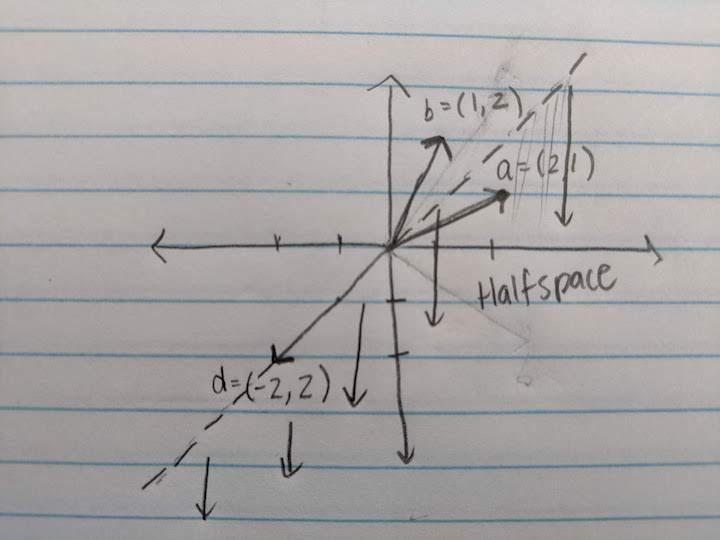
\includegraphics[scale=0.6]{figures/halfspace.jpg}
  \caption{Drawing of the half-space defined by $a$ and $b$. Also includes the vector $c$ computed explicitly.}
  \label{fig:halfspace_drawing}
\end{figure}

\newpage
\Q{Linearizing range measurements}
\begin{solution}
  \begin{enumerate}[label=(\alph*)]
    \item
      We first derive the linearization analytically. We have $f: \mathbb{R}^n \to \mathbb{R}$ defined as $y = f(x) = ||x - a||$. Let us compute $Df(x)$:

      \begin{align*}
        Df(x)_{i} &= \frac{\partial f}{\partial x_i} \\
        &= \frac{\partial}{\partial x_i}\left[\sqrt{ \sum_{i} (x_i - a_i)^2 } \right]  \\
        &= \frac{x_i - a_i}{\sqrt{ \sum_{i} (x_i - a_i)^2 }} \\
        &= \frac{x_i - a_i}{|| x - a ||}
      \end{align*}
      Evaluating at $x_0$, we have:
      \[
        Df(x_0) = \frac{x_0 - a}{|| x_0 - a ||}
      \]
      which is simply the unit vector of length $1$ pointing from $a$ to $x_0$, as desired.

      Stating it fully, we have our linearized model as:
      \begin{align*}
        \delta y &= Df(x_0) \delta x \\
        &= \frac{x_0 - a}{||x_0 - a||} \delta x \tag{Shown above} \\
        &= k^T\delta x \tag{Where $k$ is a unit vector pointing from $a$ to $x_0$}
      \end{align*}
      For $\mathbb{R}^2$, we can visualize the above as shown in Figure \ref{fig:visualizations_single_beacon_r2}.
    \item We proceed now to show the following:
    \[
      0 \leq \eta \leq \frac{\alpha^2}{2}
    \]
    where:
    \[
      \eta = \frac{||x_0 + \delta x - a|| - ||x_0 - a|| - k^T \delta x}{||x_0 - a||}
    \]
    is our relative error of the approximation from above
    and:
    \[
      \alpha = \frac{||\delta x||}{|| x_0 - a||}
    \]
    is the relative size of $\delta x$.

    We do this step-by-step as described in the problem statement. First, we begin by showing the following:
    \[
      \eta = -1 + \sqrt{1 + \alpha^2 + 2\beta} - \beta
    \]
    where $\beta = \frac{ k^T \delta x }{|| x_0 - a||}$.

    We show this result directly:
    \begin{align*}
      \eta &= \frac{||x_0 + \delta x - a|| - ||x_0 - a|| - k^T \delta x}{||x_0 - a||} \\
      &= -1 - \beta + \frac{||x_0 + \delta x - a ||}{||x_0 - a ||} \tag{Simplification and defintion of $\beta$} \\
      &= -1 - \beta + \frac{\sqrt{(x_0 - a + \delta x)^T(x_0 - a + \delta x)}}{|| x_0 - a|| } \tag{$||a|| = \sqrt{a^T a}$} \\
      &= -1 - \beta + \frac{\sqrt{ ||x_0 - a||^2 + ||\delta x ||^2 + (x_0 - a)^T\delta x + \delta x^T (x_0 - a)  }}{||x_0 - a||} \tag{Multiplying it out} \\
      &= -1 - \beta + \frac{\sqrt{ ||x_0 - a||^2 + ||\delta x ||^2 + 2(x_0 - a)^T\delta x }}{||x_0 - a||} \tag{$\delta x^T (x_0 - a)$ is a scalar } \\ 
      &= -1 - \beta + \sqrt{ 1 + \left(\frac{||\delta x ||}{|| x_0 - a ||}\right)^2 + \frac{2(x_0 - a)^T\delta x}{||x_0 -a||^2} } \tag{Moving denominator into square root}\\
      &=-1 - \beta + \sqrt{ 1 + \alpha^2 + \frac{2k^T\delta x}{||x_0 - a||} } \tag{Subtitution of $\alpha$ and $k$} \\
      &= -1 - \beta + \sqrt{1 + \alpha^2 + 2\beta} \tag{Subtitution of $\beta$}
    \end{align*}

    Next, we verify that $|\beta| \leq \alpha$:
    \begin{align*}
      |\beta| &= \frac{|k^T\delta x|}{||x_0 - a||} \\
      &\leq \frac{||k|| \cdot || \delta x ||}{||x_0 - a||} \tag{By the Cauchy-Schwarz inequality} \\
      &= \frac{||\delta x||}{|| x_0 - a||} \tag{$k$ is a unit vector} \\
      &= \alpha
    \end{align*}

    We now consider the function $g(\beta) = \eta$, and try to find the minimum and maximum. Taking the derivative and setting to zero, we have:
    \begin{align*}
      \frac{dg(\beta)}{d\beta} = -1 + \frac{1}{\sqrt{1 + \alpha^2 + 2\beta}}  = 0 \\
      \implies \beta = -\frac{\alpha^2}{2}
    \end{align*}
    We now compute $g(\beta)$ at this point as well as the boundaries:
    \begin{align*}
      g(-\frac{\alpha^2}{2}) &= \frac{\alpha^2}{2} \\
      g(-\alpha) &= -1 + \sqrt{(1 + \alpha)^2} - \alpha = 0\\
      g(\alpha) &= 0
    \end{align*}
    With the above, we now conclude knowing that on the interval $-\alpha \leq \beta < \alpha$, we have $0 \leq g(\beta) \leq \frac{\alpha^2}{2}$. This proves the bound on our error.
  \end{enumerate}
\end{solution}
\begin{figure}[!ht]
  \centering
  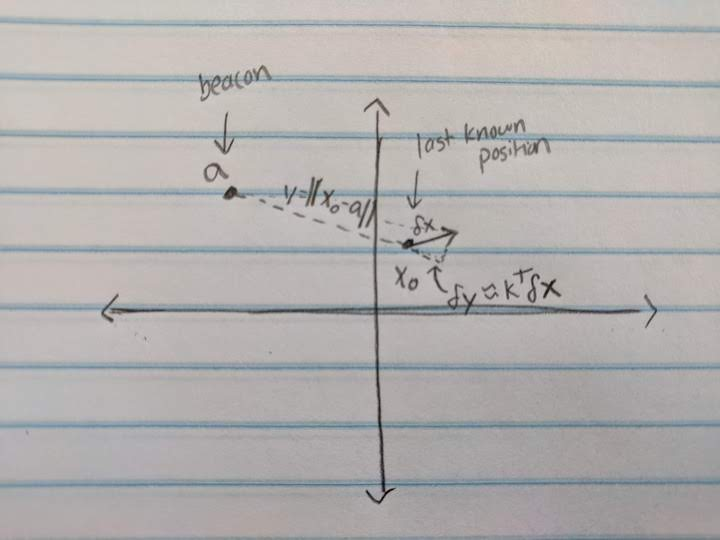
\includegraphics[scale=0.6]{figures/single_beacon.jpg}
  \caption{A small change $\delta x$ leads to $\delta y$ which is approximated by the projection of $\delta x$ onto the unit vector from from $a$ to $x_0$.}
  \label{fig:visualizations_single_beacon_r2}
\end{figure}

\newpage
\Q{Orthogonal complement of a subspace}
\begin{solution}
  \begin{enumerate}[label=(\alph*)]
    \item We verify that $\mathcal{V}^{\perp}$ is a subspace of $\mathbb{R}^n$. We do this by showing that it is closed under addition and scalar multiplication.

    Consider $x, z \in \mathcal{V}^{\perp}, a,b \in \mathbb{R}$. We show that $ax + bz \in \mathcal{V}^{\perp}$. To do this, we need to show that $\langle ax + bz, y \rangle = 0, \forall y \in \mathcal{V}$.
    \begin{align*}
      \langle ax + bz, y \rangle &= a\langle x, y\rangle + b\langle x, z \rangle \tag{Linearity of dot product} \\
      &= 0 + 0 \tag{$x,y \in \mathcal{V}^{\perp}$} 
    \end{align*}
    This concludes our proof.

    \item $\mathcal{V} = \textbf{range}(V)$, since by definition the range of $V$ is the span of its columns. On the other hand, $\mathcal{V}^{\perp}$ is $\textbf{null}(V)$ since the nullspace is the set of vectors which are orthogonal to all vectors in the image of $V$.

    \item Take $x \in \mathbb{R}^n$ and wish to prove that $x = v + v^{\perp}$ where $v \in \mathcal{V}$ and $v^{\perp} \in \mathcal{V}^{\perp}$. As the hint indicates, let's take $P = V(V^T V)^{-1}V$ be the projection matrix onto the space $\mathcal{V}$ as discussed in class. Then let $v = Px$ and take $v^{\perp} = x - Px = (I - P)x$ (it is clear that $x = v + v^{\perp}$). Since $P$ is the projection operator onto $\mathcal{V}$, we immediately have that $v \in \mathcal{V}$. We now show that $v^{\perp} \in \mathcal{V}^{\perp}$. Consider what happens when we apply the projection operation $P$ to $v^{\perp}$:
    \begin{align*}
      Pv^{\perp} &= P(I - P)x \\
      &= (P - P^2)x \\
      &= (P - P)x \tag{$P^2 = P$ since a projection applied twice is the same as applied once} \\
      &= 0
    \end{align*}
    From the above, it is clear that $v^{\perp} \in \textbf{image}(P)^{\perp} = \mathcal{V}^{\perp}$, as discussed in (b).

    The next step is to show that this decomposition is unique.

    Let there be some other decomposition $x = u + w$ where $u \in \mathcal{V}, w \in \mathcal{V}^{\perp}$. We now show that $u = v$ and $w = v^{\perp}$, meaning our decomposition is unque. We have that $v = Px = P(u + w) = Pu + 0 = u$, so $u = v$. Using this, we also have that $w = x - u = x - v = v^{\perp}$. Therefore the decomposition is unique.
    \item This follows almost immediately from (b). 
    \begin{align*}
        \text{dim } \mathcal{V}^{\perp} + \text{dim } \mathcal{V} &= \text{dim } \textbf{range}(V) + \text{dim } \textbf{null}(V) \\
        &= \text{dim } \mathbb{R}^n \tag{By Rank-nullity theorem} \\
        &= n
      \end{align*}
    \item We wish to show that given $\mathcal{V} \subseteq \mathcal{U} \implies \mathcal{U}^T \subseteq \mathcal{V}^{\perp}$.

    Take any $x \in \mathcal{U}^T$. By definition of orthogonal complement, we must have that $\langle x, y \rangle = 0, \forall y \in \mathcal{U}$. However, since $\mathcal{V} \subseteq \mathcal{U}$, this implies that $\langle x, z \rangle = 0, \forall z \in \mathcal{V}$. This further implies that $x \in \mathcal{V}^{\perp}$, concluding the proof.
  \end{enumerate}
\end{solution}

\newpage
\Q{Single sensor failure detection and identification}

\begin{solution}
A single sensor failed. The failing sensor is sensor the 11-th sensor (the sensor at index $10$). 

First, no sensor failed if $\tilde{y} \in \textbf{span}(A)$. We can check this by checking to see if $\textbf{rank}(A) == \textbf{rank} \left(\begin{bmatrix} A & \tilde{y} \end{bmatrix}\right)$ (we add $\tilde{y}$ as a column to $A$ and see if the ranks changes).

If the rank does not change, this means that there are no failing sensors.

If the rank is different, then we must have at least one failing sensor. The problem statement makes it clear that a single sensor failed. As such, we can just go through and check each sensor. 

Let $A_{-i} \in \mathbb{R}^{(m-1) \times n}$ be the matrix $A$ but with row $i$ removed, and similarly, let $\tilde{y}_{-i} \in \mathbb{R}^{m-1}$ be $\tilde{y}$ but with the $i$-th entry missing.

Then we know that $\textbf{rank}(A_{-i}) == \textbf{rank}\left( \begin{bmatrix} A_{-i} & \tilde{y}_{-i} \end{bmatrix}\right)$ if and only if $\tilde{y}_{-i} \in \textbf{span}(A_{-i})$ which implies that $i$ is the failing sensor (since ignoring it leads to a consistent solution).

Following the process described above, we determined that for the given $A$ and $\tilde{y}$, the failing sensor is the $11$-th sensor, the sensor corresponding to row $11$ in matrix $A$, one-indexed.
\end{solution}

\newpage
\Q{Reverse engineering a smoothing filter}

\begin{solution}
  \begin{enumerate}[label=(\alph*)]
    \item Taking the derivative of $J$ with respect to $y_i$, we have:
    \begin{align*}
      \frac{\partial J^{\text{track}}}{\partial y_i} &= -2(u_i - y_i) \\
      \frac{\partial J^{\text{norm}}}{\partial y_i} &= 2y_i \\
      \frac{\partial J^{\text{cont}}}{\partial y_i} &= 
      \begin{cases}
      - 2(y_{i+1} - y_{i}) & i = 1 \\
        2(y_i - y_{i-1}) & i = n \\
        2(y_i - y_{i-1}) - 2(y_{i+1} - y_{i}) & \text{otherwise}
      \end{cases} \\
      \frac{\partial J^{\text{smooth}}}{\partial y_i} &= 
      \begin{cases}
          2(y_{i+2} - 2y_{i+1} + y_{i}) & i = 1 \\
          -4(y_{i+1} - 2y_{i} + y_{i-1}) & i = 2, n = 3\\
          2(y_{i+2} - 2y_{i+1} + y_{i}) - 4(y_{i+1} - 2y_{i} + y_{i-1}) & i = 2, n > 3 \\
          2(y_{i} - 2y_{i-1} + y_{i-2}) - 4(y_{i+1} - 2y_{i} + y_{i-1}) & i = n - 1, n > 3 \\
          2(y_{i} - 2y_{i-1} + y_{i-2}) & i = n \\
          2(y_{i+2} - 2y_{i+1} + y_{i}) - 4(y_{i+1} - 2y_{i} + y_{i-1}) + 2(y_i - 2y_{i-1} + y_{i-2}) & \text{otherwise}
      \end{cases}
    \end{align*}
    Plugging into the equation given and setting equal to $0$ (and simplifying), we have that:
    \begin{align*}
      \lambda y_i - \mu(y_{i+1} - y_i) + \kappa(y_{i+2} - 2y_{i+1} + y_i) = u_i - y_i \tag{$i = 1$} \\
      \lambda y_i + \mu(2y_i - y_{i+1} - y_{i-1}) + \kappa(-2y_{i+1} + 4y_{i} -2y_{i-1}) = u_i - y_i \tag{$i=2, n = 3$} \\
      \lambda y_i + \mu(2y_i - y_{i+1} - y_{i-1}) + \kappa(y_{i+2} - 4y_{i+1} + 5y_{i} -2y_{i-1} ) = u_i - y_i \tag{$i = 2, n > 3$} \\
      \lambda y_i + \mu(2y_i - y_{i+1} - y_{i-1}) + \kappa(-2y_{i+1} + 5y_i -4y_{i-1} + y_{i-2}) = u_i - y_i \tag{$i = n - 1, n > 3$} \\
      \lambda y_i - \mu(y_i - y_{i-1}) + \kappa(y_i - 2y_{i-1} + y_{i-2}) = u_i - y_i \tag{$i = n$} \\
      \lambda y_i + \mu(2y_i - y_{i+1} - y_{i-1}) + \kappa (y_{i+2} - 4y_{i+1} - 6y_i - 4y_{i-1} + y_{i-2}) &= u_i - y_i \tag{otherwise}
    \end{align*}
    which we can write in matrix form as:
    \[
      A\begin{bmatrix}
        \lambda \\ \mu \\ \kappa
      \end{bmatrix} = u - y
    \]
    where 
    \begin{align*}
      A &= \begin{bmatrix}
        y_1 & -(y_{2} - y_1) & (y_{3} - 2y_{2} + y_1) \\
        y_2 & 2y_2 - y_{3} - y_{1} & y_{4} - 4y_{3} + 5y_{2} -2y_{1} \\
        & \vdots & \\
        y_i & 2y_i - y_{i+1} - y_{i-1} & y_{i+2} - 4y_{i+1} - 6y_i - 4y_{i-1} + y_{i-2} \\
        & \vdots & \\
        y_{n-1} & 2y_{n-1} - y_{n} - y_{n-2} & -2y_{n} + 5y_{n-1} -4y_{n-2} + y_{n-3} \\
        y_n & -(y_n - y_{n-1}) & y_n - 2y_{n-1} + y_{n-2}
      \end{bmatrix}  \tag{$n > 3$} \\
      A &= 
      \begin{bmatrix}
        y_1 & -(y_{2} - y_1) & y_{3} - 2y_{2} + y_1 \\
        y_2 & 2y_2 - y_{3} - y_{1} & -2y_3 + 4y_2 - 2y_1) \\
        y_3 & -(y_3 - y_{2}) & y_3 - 2y_{2} + y_1)
      \end{bmatrix} \tag{$n = 3$}
    \end{align*}
    Since we know that a solution exists and that $n \geq 3$, we can always solve the above system of equations by forming a smaller $B \in \mathbb{R}^{3 \times 3}$ formed from any $3$ rows of $A$. For example, we can form the matrix:
    \[
      B =
        \begin{bmatrix}
          y_2 & 2y_2 - y_{3} - y_{1} & y_{4} - 4y_{3} + 5y_{2} -2y_{1} \\
          y_3 & 2y_3 - y_{4} - y_{2} & y_{5} - 4y_{4} + 5y_{3} -2y_{2} \\
          y_4 & 2y_4 - y_{5} - y_{3} & y_{6} - 4y_{5} + 5y_{4} -2y_{3} \\
        \end{bmatrix}
    \]
    We can check that \textbf{rank}$(B) = 3$\footnote{See code for details}, so $B$ is invertible. If not, we can pick another set of $3$ rows.
    We can then simply solve the following:
    \[
      \begin{bmatrix}
        \lambda \\
        \mu \\
        \kappa 
      \end{bmatrix} = B^{-1}
      \begin{bmatrix}
        u_3 - y_3 \\
        u_4 - y_4 \\
        u_5 - y_5
      \end{bmatrix}
    \]
    which will give us the values of our constants.

    \item
      We now carry out the process described above using the provided $y$ and $u$ vectors. See the attached code for details. We end up with:
      \[
        B^{-1}\begin{bmatrix}
        u_3 - y_3 \\
        u_4 - y_4 \\
        u_5 - y_5
      \end{bmatrix} = 
      \begin{bmatrix}
        120.09994427 \\
        2.00001039 \\
        9.99999534
      \end{bmatrix} \approx
      \begin{bmatrix}
        120.1 \\
        2 \\
        10
      \end{bmatrix} 
      \]
  \end{enumerate}
\end{solution}

\newpage
\Q{Estimating link delays from route latencies}

\begin{solution}
  Optional. Skip.
\end{solution}

\newpage
\Q{Trace of a square matrix}
\begin{solution}
\begin{enumerate}[label=(\alph*)]
  \item We show that for $A,B \in \mathbb{R}^n$, $\text{trace}(AB) = \text{trace}(BA)$.
  \begin{align*}
    \text{trace}(AB) &= \sum_{i = 1}^n (AB)_{ii} \tag{Definition of trace} \\
    &= \sum_{i=1}^n \sum_{k=1}^n A_{ik}B_{ki} \tag{Definition of matrix multiplication} \\
    &= \sum_{k=1}^n \sum_{i=1}^n B_{ki}A_{ik} \tag{Swap summation indexes and use commutativity of scalar multiplication} \\
    &= \sum_{k=1}^n (BA)_{kk} \tag{Definition of matrix multiplication} \\
    &= \text{trace}(BA) \tag{Definition of trace}
  \end{align*}
  \item We can compute $||A||$ directly as follows:
  \begin{align*}
    ||A|| &= \{\text{trace}(AA^T)\}^{\frac{1}{2}} \\
    &= \sqrt{\sum_{i=1}^n (AA^T)_{ii}} \tag{Definition of trace} \\
    &= \sqrt{\sum_{i=1}^n \sum_{j=1}^n A_{ij}^2 } \tag{Definition of matrix multiplication}
  \end{align*}
  That is to say, $||A||$ is simply the square root of the sum of squares of the entries of $A$.
  \item We show that $\langle A, B \rangle = \text{vec}(A)^T \vec{B}$. 
  \begin{align*}
    \langle A, B \rangle &= \text{trace}(AB^T) \tag{Given in part (b)} \\
    &= \sum_{i=1}^n (AB^T)_{ii} \tag{Definition of trace} \\
    &= \sum_{i=1}^n \sum_{j=1}^n A_{ij}B_{ij} \tag{Definition of matrix multiplication} \\
    &= \sum_{j=1}^n \left( \sum_{i=1}^n A_{ij}B_{ij} \right) \tag{Swap indeces to show that we're multiplying elements in corresponding columns and summing them} \\
    &= \sum_{k=1}^{n^2} \text{vec}(A)_k \text{vec}(B)_k \tag{Re-indexing and using definition of vec($\cdot$)} \\
    &= \text{vec}(A)^T \text{vec}(B) \tag{Definition of dot product}
  \end{align*}

\end{enumerate}
\end{solution}

\newpage
\Q{Zeroing out the board}
\begin{solution}
  \begin{enumerate}[label=(\alph*)]
    \item 
      Essentially, Reze is trying to find a linear combination of basis vectors (to be defined later) which constructs the $6 \times 6$ board that Bobbie provides.

      In fact, our basis vectors are of the form:
      \begin{align*}
        v_{11} &= 
          \begin{bmatrix}
            1 & -1 & 0 & 0 & 0 & 0 \\
            -1 & 0 & 0 & 0 & 0 & 0 \\
            0 & 0 & 0 & 0 & 0 & 0 \\
            0 & 0 & 0 & 0 & 0 & 0 \\
            0 & 0 & 0 & 0 & 0 & 0 \\
            0 & 0 & 0 & 0 & 0 & 0 \\
          \end{bmatrix} \\
          v_{12} &= 
          \begin{bmatrix}
            -1 & 1 & -1 & 0 & 0 & 0 \\
            0 & -1 & 0 & 0 & 0 & 0 \\
            0 & 0 & 0 & 0 & 0 & 0 \\
            0 & 0 & 0 & 0 & 0 & 0 \\
            0 & 0 & 0 & 0 & 0 & 0 \\
            0 & 0 & 0 & 0 & 0 & 0 \\
          \end{bmatrix} \\
          & \vdots \\
          v_{33} &= 
            \begin{bmatrix}
            0 & 0 & 0 & 0 & 0 & 0 \\
            0 & 0 & -1 & 0 & 0 & 0 \\
            0 & -1 & 1 & -1 & 0 & 0 \\
            0 & 0 & -1 & 0 & 0 & 0 \\
            0 & 0 & 0 & 0 & 0 & 0 \\
            0 & 0 & 0 & 0 & 0 & 0 \\
          \end{bmatrix} \\
          & \vdots
      \end{align*}
      Using the vectorize function defined in Problem 8, we can vectorize each of the above so that we have $\text{vec}(v_{ij} = v_k \in \mathbb{R}^{36}$ where $k = i \times j$. 
      
      In this context, the vector given by Bobbie is (assuming a $1$ is placed at position $(1,1)$)
      \[
        x = \begin{bmatrix}
          1 \\
          0 \\
          \vdots
        \end{bmatrix} \in  \mathbb{R}^{36}
      \]
      and the question simply boils down to whether $x \in \textbf{span}(\{v_k\})$. We can programatically verify that $\textbf{span}(\{v_k\}) = \mathbb{R}^{36}$, which means that Reza can win the game.

      In fact, by computing $A^{-1} x$, we can determine the exact set of actions which Reza should take. The actions are given by the matrix below, where the value within each cell corresponds to the real number that Reza should pick to add to that cell (and subtract from adjacent cells). Note that the numbers are truncated here, but see the code snippet for the full output.

      \[
        \begin{bmatrix}
          -1.3076 &  -0.15384 & 0.69230 &  0.46153 &  -0.076923 & -0.23076 \\ 
        0.15384 & 0.46153 & 0.38461 & -0.15384 & -0.30769 & -0.15384 \\
        0.69230 & 0.38461 & -0.61538 & -0.69230 & 0.076923 & 0.38461 \\
       0.46153 & -0.15384 & -0.69230 & 0 & 0.69230 & 0.46153 \\
       -0.076923 & -0.30769 & 0.076923 & 0.69230 & 0.15384 & -0.61538 \\
        -0.23076 & -0.15384 & 0.38461 & 0.46153 & -0.61538 & -1.2307
        \end{bmatrix}
      \]

      \item Bobbie cannot fill in the table so that Reza has no possible way of solving it. This is becase, as shown in part (a) and as computed programatically, we have that $\textbf{rank}\left( \begin{bmatrix} v_1 & \cdots & v_{36} \end{bmatrix} \right) = 36$, meaning that $\textbf{span}(\{v_k\}) = \mathbb{R}^{36}$, and as such, no matter what the initial vector $y \in \mathbb{R}^36$ is that Bobbie constructs, Reza can always compute:
      $$
        x = A^{-1}y \in \mathbb{R}^{36}
      $$
      and Reza can then, for each $k = 1, \cdots, 36$ simply pick cell $(i,j)$ and the real number $-x_k$ as her action, where $i = \lceil k / 6 \rceil$ and $j = [(k - 1) \mod 6] + 1$. Since $x$ is exactly the coefficients that lead to $y$, their negation will zero out the initial vector.

      \item Interestingly enough, for a $9 \times 9$ board, we have that $\text{dim }\textbf{span}(\{v_k\}) = 79$, meaning that the actions which Reza can take (the basis vectors) do not span the entire space (which is $\mathbb{R}^{81}$). 

      Using Python and Numpy \footnote{See attached code}, we can compute this nullspace. As such, we know that the following board cannot be solved by Reza, since this board lies in the null-space.
      \[
        \begin{bmatrix}
           0 & 1 & 1 & 0 & 0 & 0 & 0 & 0 & 0 \\
           0 & 0 & 0 & 0 & 0 & 1 & 0 & 0 & 1 \\
           0 & 0 & 0 & 0 & 0 & 1 & 0 & 0 & 1 \\
           0 & 1 & 1 & 0 & 0 & 0 & 0 & 0 & 0 \\
           0 & 0 & 0 & 0 & 0 & 0 & 0 & 0 & 0 \\
           0 & 0 & 0 & 0 & 0 & 0 & 1 & 1 & 0 \\
           1 & 0 & 0 & 1 & 0 & 0 & 0 & 0 & 0 \\
           1 & 0 & 0 & 1 & 0 & 0 & 0 & 0 & 0 \\
           0 & 0 & 0 & 0 & 0 & 0 & 1 & 1 & 0
       \end{bmatrix}
      \]
  \end{enumerate}
\end{solution}


\end{questions}


\includepdf[
    %% Include all pages of the PDF
    pages=-,
    %% make this page have the usual page style
    %% (you can change it to plain etc). By default pdfpages
    %% sets the pagecommand to \pagestyle{empty}
    pagecommand={\pagestyle{headings}}]
%% The pdf file itself
{HW2.pdf}























\end{document}
